%%%%%%%%%%%%%%%%%%%%%%%%%%%%%%%%%%%%%%%%%
% Short Sectioned Assignment LaTeX Template Version 1.0 (5/5/12)
% This template has been downloaded from: http://www.LaTeXTemplates.com
% Original author:  Frits Wenneker (http://www.howtotex.com)
% License: CC BY-NC-SA 3.0 (http://creativecommons.org/licenses/by-nc-sa/3.0/)
%%%%%%%%%%%%%%%%%%%%%%%%%%%%%%%%%%%%%%%%%

%----------------------------------------------------------------------------------------
%	PACKAGES AND OTHER DOCUMENT CONFIGURATIONS
%----------------------------------------------------------------------------------------

\documentclass[paper=a4, fontsize=11pt]{scrartcl} % A4 paper and 11pt font size

% ---- Entrada y salida de texto -----

\usepackage[T1]{fontenc} % Use 8-bit encoding that has 256 glyphs
\usepackage[utf8]{inputenc}
%\usepackage{fourier} % Use the Adobe Utopia font for the document - comment this line to return to the LaTeX default

% ---- Idioma --------

\usepackage[spanish, es-tabla]{babel} % Selecciona el español para palabras introducidas automáticamente, p.ej. "septiembre" en la fecha y especifica que se use la palabra Tabla en vez de Cuadro

\usepackage{eurosym}
\usepackage{enumitem}

% ---- Otros paquetes ----

\usepackage{url} % ,href} %para incluir URLs e hipervínculos dentro del texto (aunque hay que instalar href)
\usepackage{amsmath,amsfonts,amsthm} % Math packages
%\usepackage{graphics,graphicx, floatrow} %para incluir imágenes y notas en las imágenes
\usepackage{graphics,graphicx, float} %para incluir imágenes y colocarlas

% Para hacer tablas comlejas
%\usepackage{multirow}
%\usepackage{threeparttable}

%\usepackage{sectsty} % Allows customizing section commands
%\allsectionsfont{\centering \normalfont\scshape} % Make all sections centered, the default font and small caps

\usepackage{fancyhdr} % Custom headers and footers
\pagestyle{fancyplain} % Makes all pages in the document conform to the custom headers and footers
\fancyhead{} % No page header - if you want one, create it in the same way as the footers below
\fancyfoot[L]{} % Empty left footer
\fancyfoot[C]{} % Empty center footer
\fancyfoot[R]{\thepage} % Page numbering for right footer
\renewcommand{\headrulewidth}{0pt} % Remove header underlines
\renewcommand{\footrulewidth}{0pt} % Remove footer underlines
\setlength{\headheight}{13.6pt} % Customize the height of the header

\numberwithin{equation}{section} % Number equations within sections (i.e. 1.1, 1.2, 2.1, 2.2 instead of 1, 2, 3, 4)
\numberwithin{figure}{section} % Number figures within sections (i.e. 1.1, 1.2, 2.1, 2.2 instead of 1, 2, 3, 4)
\numberwithin{table}{section} % Number tables within sections (i.e. 1.1, 1.2, 2.1, 2.2 instead of 1, 2, 3, 4)

\setlength\parindent{0pt} % Removes all indentation from paragraphs - comment this line for an assignment with lots of text

\newcommand{\horrule}[1]{\rule{\linewidth}{#1}} % Create horizontal rule command with 1 argument of height


%----------------------------------------------------------------------------------------
%	TÍTULO Y DATOS DEL ALUMNO
%----------------------------------------------------------------------------------------

\title{	
\normalfont \normalsize 
\textsc{\textbf{Ingeniería de Servidores (2016-2017)} \\ Grado en Ingeniería Informática \\ Universidad de Granada} \\ [25pt] % Your university, school and/or department name(s)
\horrule{0.5pt} \\[0.4cm] % Thin top horizontal rule
\huge Memoria Práctica 4 \\ % The assignment title
\horrule{2pt} \\[0.5cm] % Thick bottom horizontal rule
}

\author{Cristian Vélez Ruiz} % Nombre y apellidos

\date{\normalsize\today} % Incluye la fecha actual

%----------------------------------------------------------------------------------------
% DOCUMENTO
%----------------------------------------------------------------------------------------
\begin{document}

\maketitle % Muestra el Título

\newpage %inserta un salto de página

\tableofcontents % para generar el índice de contenidos

\listoffigures

\listoftables

\newpage

%----------------------------------------------------------------------------------------
%	Cuestión 1
%----------------------------------------------------------------------------------------
\section[Cuestión 1]{Seleccione, instale y ejecute uno, comente los resultados.Atención: no es lo mismo un benchmark que una suite, instale un benchmark}

He elegido un benchmark que se centra en la renderización de graficos en Linux, su nombre es Heaven \cite{heaven}.

Ejecución Heaven Benchmark:

\begin{enumerate}
	\item Debemos ir a la pagina principal de Heaven y descargar el archivo, pesa unos 200 MiB.
	
	\begin{figure}[H] %con el [H] le obligamos a situar aquí la figura
		\centering
		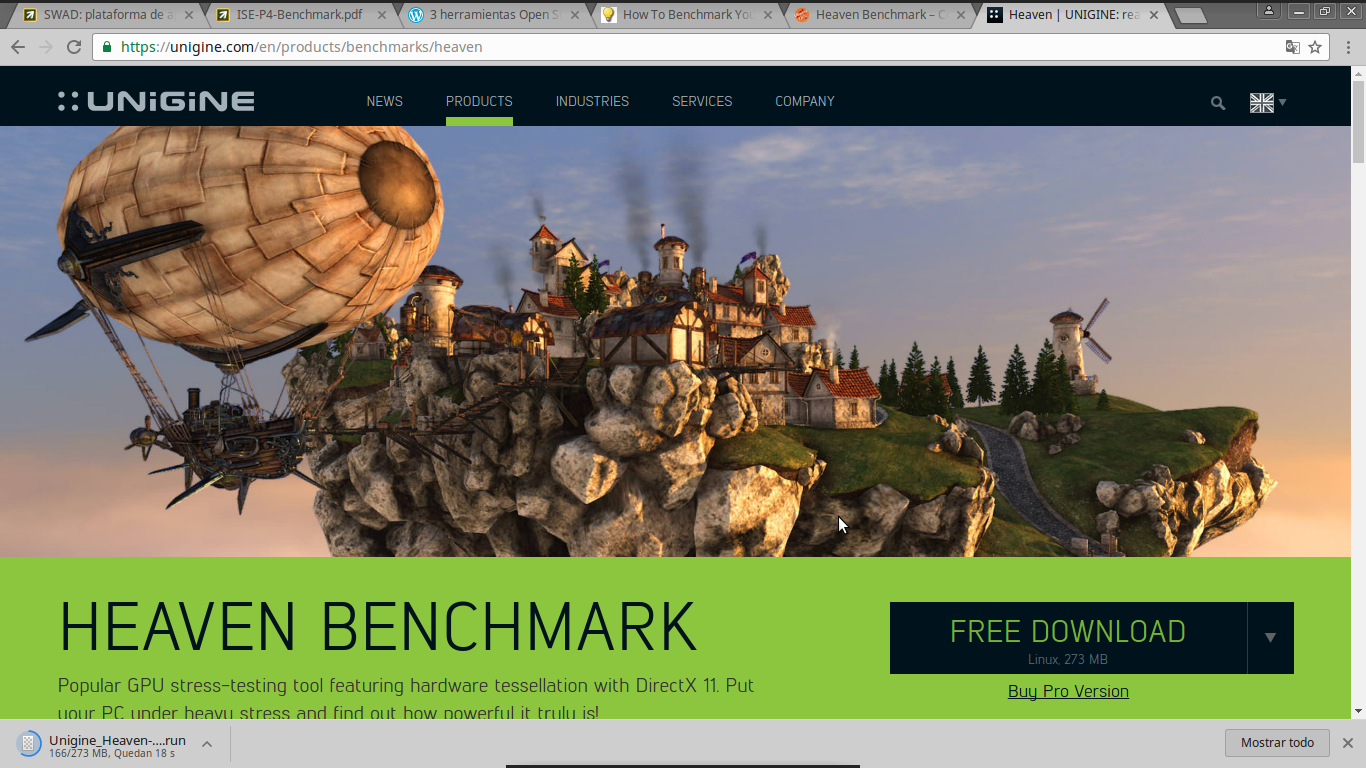
\includegraphics[scale=0.3]{pics/heaven}  %el parámetro scale permite agrandar o achicar la imagen. En el nombre de archivo puede especificar directorios
		\caption{Descargando Heaven} \label{fig:figuraDescarga}
	\end{figure}

	\item Una vez tenemos el archivo descargado tenemos que darle permisos de ejecución y ejecutarlo.
	
	\begin{figure}[H] %con el [H] le obligamos a situar aquí la figura
		\centering
		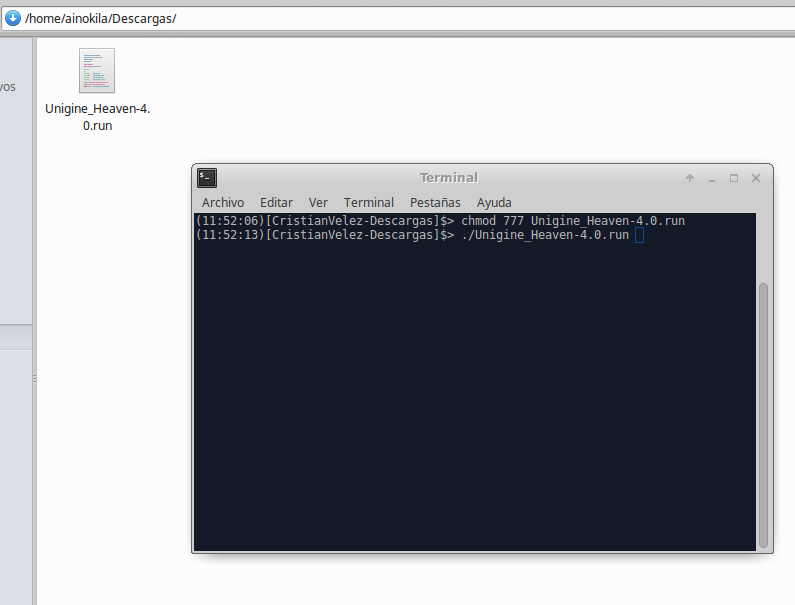
\includegraphics[scale=0.3]{pics/heaven1}  %el parámetro scale permite agrandar o achicar la imagen. En el nombre de archivo puede especificar directorios
		\caption{Desempaquetando Heaven} \label{fig:HEAVEN1}
	\end{figure}

	\begin{figure}[H] %con el [H] le obligamos a situar aquí la figura
		\centering
		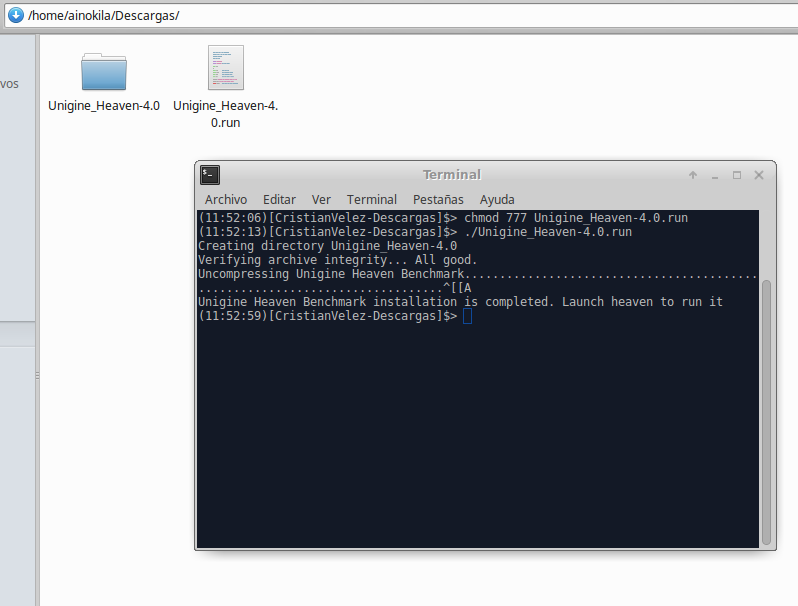
\includegraphics[scale=0.3]{pics/heaven2}  %el parámetro scale permite agrandar o achicar la imagen. En el nombre de archivo puede especificar directorios
		\caption{Listando Archivos Heaven} \label{fig:HEAVEN2}
	\end{figure}

	\item Ahora nos ha generado un directorio, en el cual debemos acceder y ejecutar \textit{./heaven}.
	
	\begin{figure}[H] %con el [H] le obligamos a situar aquí la figura
		\centering
		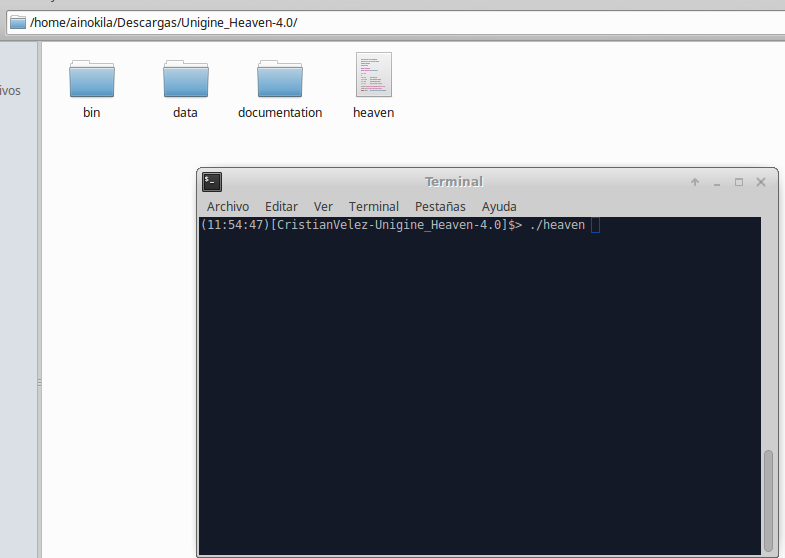
\includegraphics[scale=0.3]{pics/heaven3}  %el parámetro scale permite agrandar o achicar la imagen. En el nombre de archivo puede especificar directorios
		\caption{Ejecutando Heaven} \label{fig:HEAVEN3}
	\end{figure}

	\item Ahora se nos abrira la interfaz inicial de Heaven para configurar el benchmark, mi configuración será la siguiente:
	
	\begin{figure}[H] %con el [H] le obligamos a situar aquí la figura
		\centering
		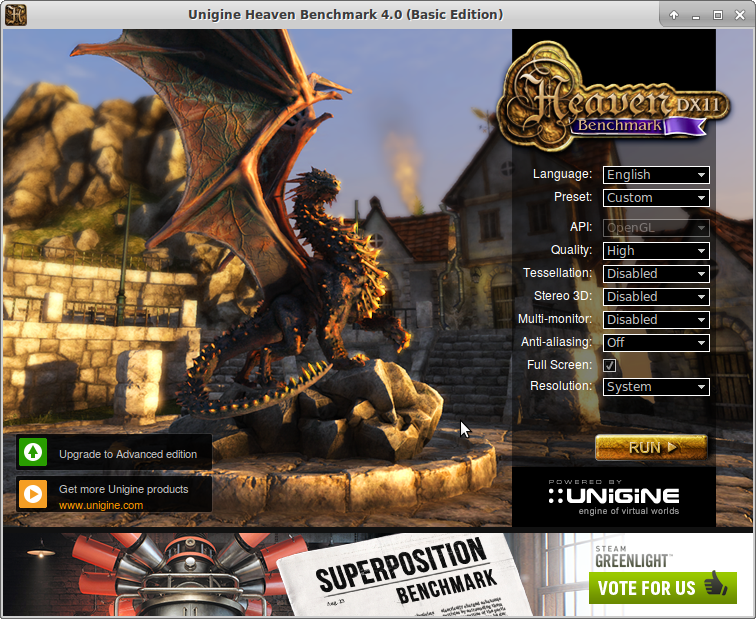
\includegraphics[scale=0.3]{pics/heaven4}  %el parámetro scale permite agrandar o achicar la imagen. En el nombre de archivo puede especificar directorios
		\caption{Configuración de Heaven} \label{fig:HEAVEN4}
	\end{figure}
	
	\item Simplemente ahora le damos a \textit{run} y cambiará la interfaz a otra y debemos seleccionar en la parte superior de arriba benchmark.
	
	\begin{figure}[H] %con el [H] le obligamos a situar aquí la figura
		\centering
		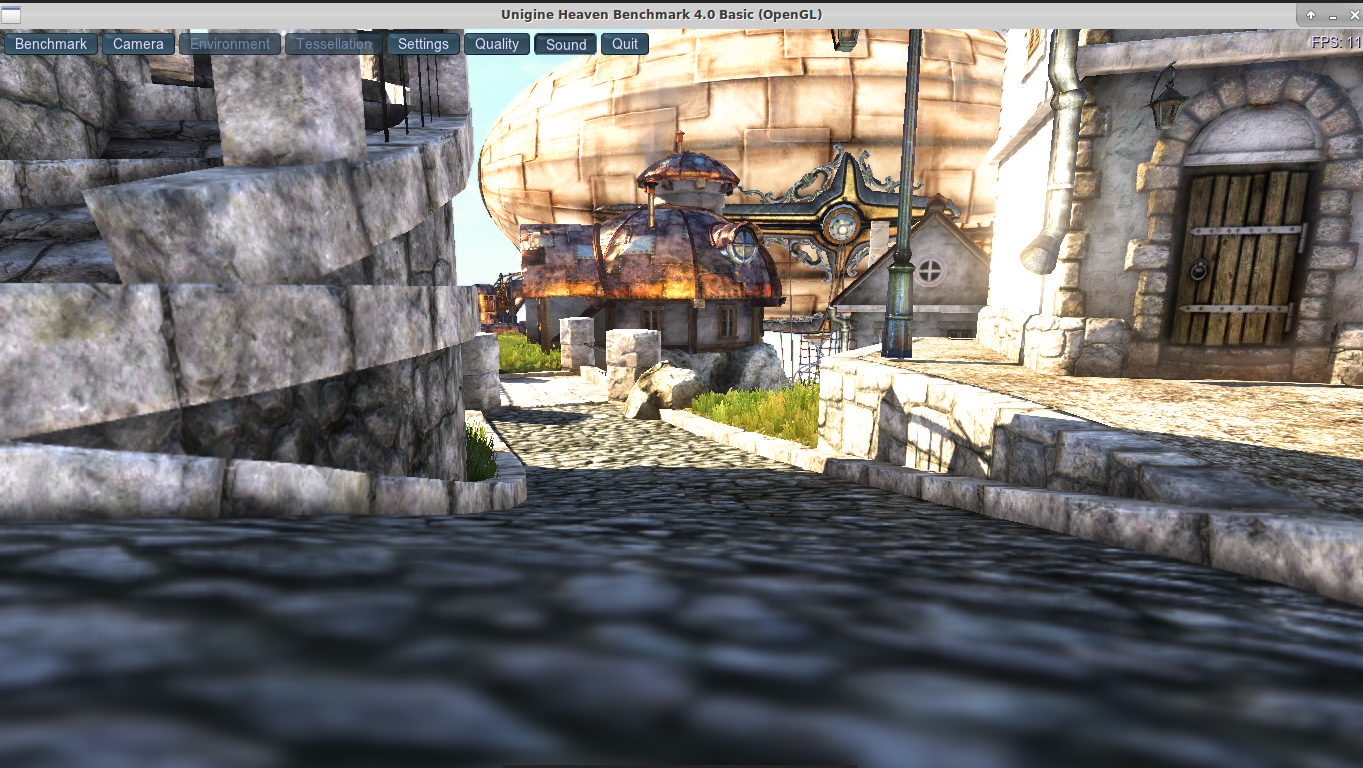
\includegraphics[scale=0.3]{pics/heaven6}  %el parámetro scale permite agrandar o achicar la imagen. En el nombre de archivo puede especificar directorios
		\caption{Iniciando benchmark} \label{fig:HEAVEN5}
	\end{figure}

	\item Una vez hemos seleccionado benchmark debemos esperar a que se generen 26 escenas distintas de las cuales luego obtendremos los resultados.
	
	\begin{figure}[H] %con el [H] le obligamos a situar aquí la figura
		\centering
		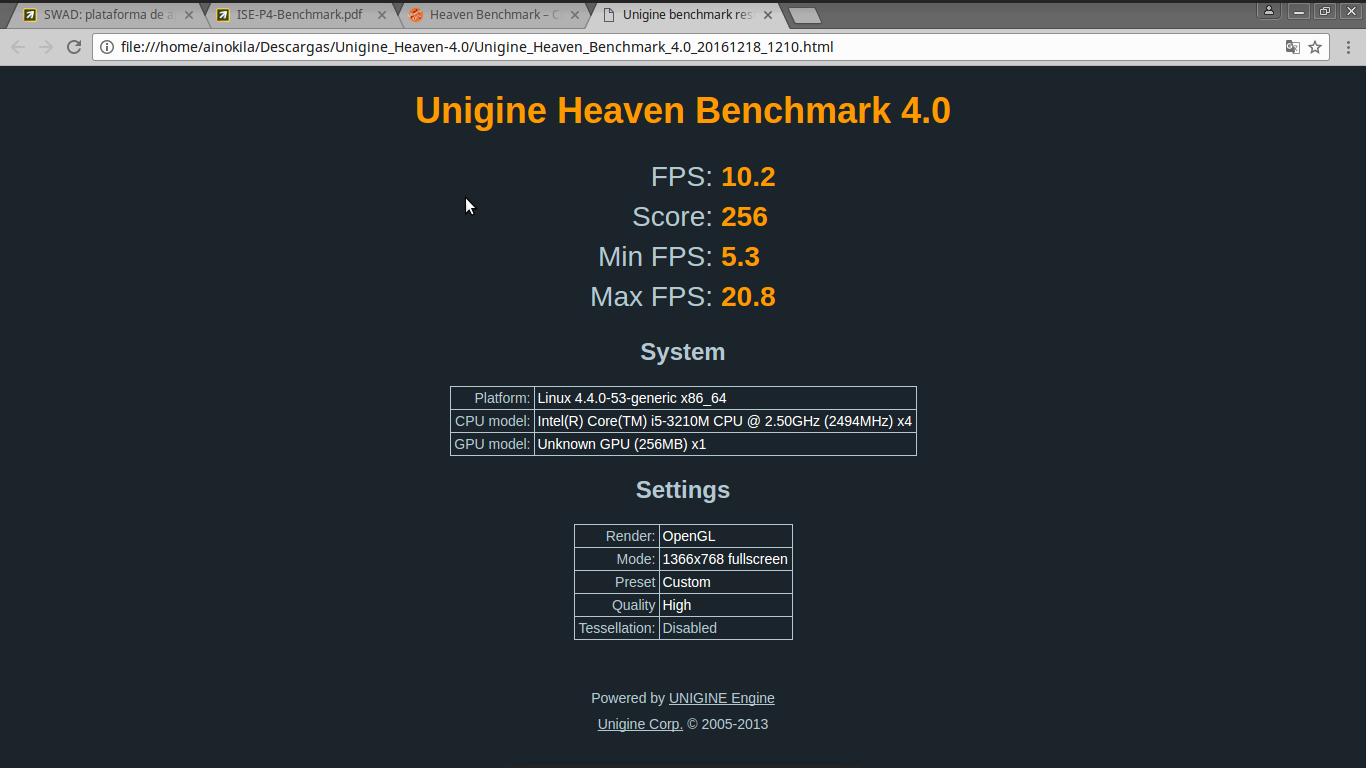
\includegraphics[scale=0.3]{pics/heaven7}  %el parámetro scale permite agrandar o achicar la imagen. En el nombre de archivo puede especificar directorios
		\caption{Resultados de Heaven} \label{fig:HEAVEN6}
	\end{figure}

	\item Los resultados de ejecutar Heaven en mi maquina portátil han sido que ha obtenido una generación media de fotogramas por segundo de 10.2, una puntuación de 256, también nos informa de cuales ha sido su pico máximo y minimo de fotogramas por segundo, en este caso 20.8 y 5.3.\\
	Después simplemente nos informa de el tipo de plataforma donde se ha ejecutado y en que CPU-GPU y también la configuración del renderizado.
	
\end{enumerate}

Este tipo de Benchmark nos sirve para hacer comparaciones de distintas tarjetas gráficas con la facilidad de poder realizar la ejecución en Linux.



%----------------------------------------------------------------------------------------
%	Cuestión 2
%----------------------------------------------------------------------------------------
\section[Cuestión 2]{De los parámetros que le podemos pasar al comando ¿Qué significa -c 5 ? ¿y -n 100? Monitorice la ejecución de ab contra alguna	máquina (cualquiera) ¿cuántas “tareas” crea ab en el cliente?}

El parámetro \textbf{-c 5} indica que vamos a enviar las peticiones en grupos de 5 y con el parámetro \textbf{-n 100} indicamos el numero de peticiones totales que vamos a enviar en este caso 100 peticiones.



%----------------------------------------------------------------------------------------
%	Cuestión 3
%----------------------------------------------------------------------------------------
\section[Cuestión 3]{Ejecute ab contra a las tres máquinas virtuales (desde el SO	anfitrión a las máquina virtuales de la red local) una a una (arrancadas por	separado).¿Cuál es la que proporciona mejores resultados? Muestre y coméntelos. (Use como máquina de referencia Ubuntu Server para la comparativa).}

En mi caso para poder ejecutar el benchmark de Apache en Windows 10 debo instalar XAMPP, es una distribución de Apache que tambien contiene algunas bases de datos para poder instalarlas.\\

Instalando XAMPP:

\begin{enumerate}
	
	\item Primero debemos ir a la página principal de XAMPP \cite{xampp} y lo descargamos.
	
	\begin{figure}[H] %con el [H] le obligamos a situar aquí la figura
		\centering
		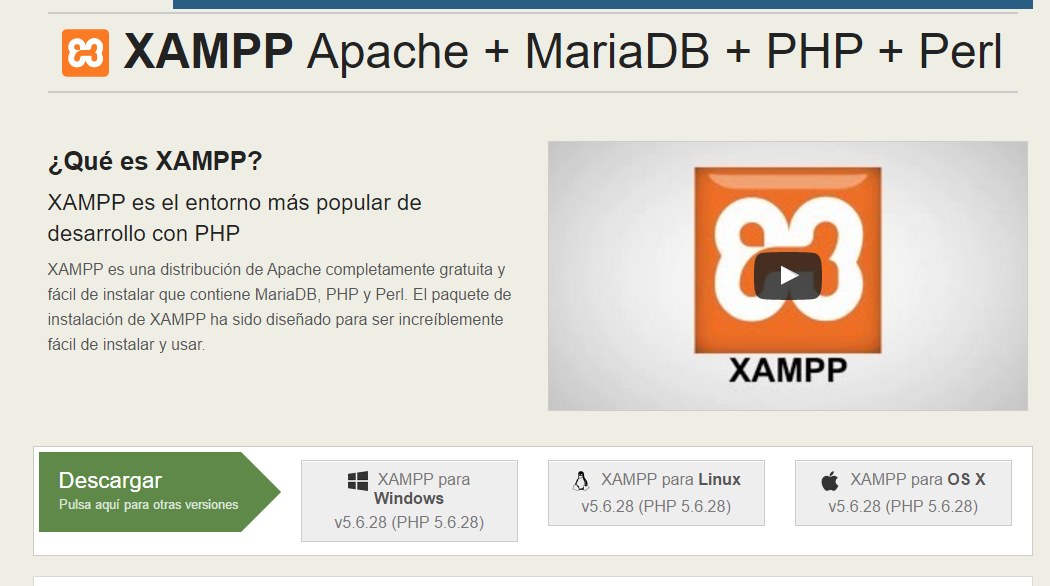
\includegraphics[scale=0.3]{pics/xampp1}  %el parámetro scale permite agrandar o achicar la imagen. En el nombre de archivo puede especificar directorios
		\caption{Página de XAMPP} \label{fig:XAMPP1}
	\end{figure}
	
	\item Ahora lo ejecutamos y damos a next.
	
	\begin{figure}[H] %con el [H] le obligamos a situar aquí la figura
		\centering
		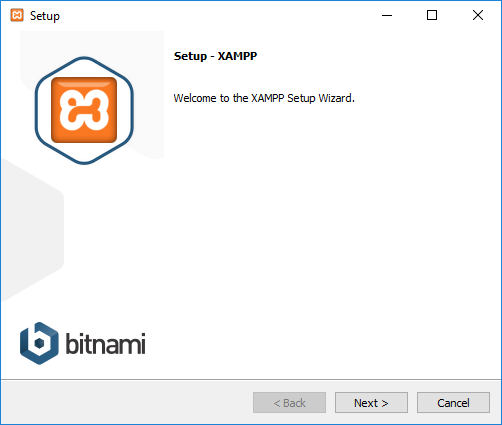
\includegraphics[scale=0.4]{pics/xampp2}  %el parámetro scale permite agrandar o achicar la imagen. En el nombre de archivo puede especificar directorios
		\caption{Paso 1 instalación XAMPP} \label{fig:XAMPP2}
	\end{figure}
	
	\item Seleccionamos los componentes que queremos instalar, en mi caso Apache, PHP y phpMyAdmin.
	
	\begin{figure}[H] %con el [H] le obligamos a situar aquí la figura
		\centering
		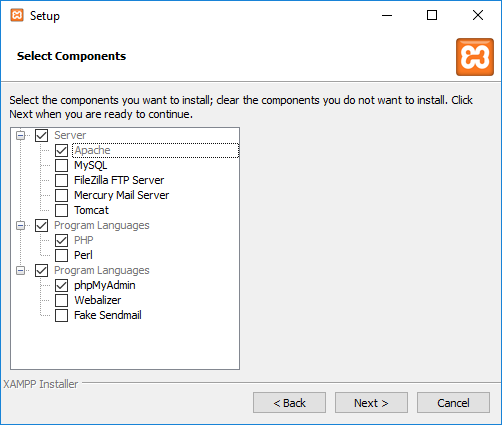
\includegraphics[scale=0.4]{pics/xampp3}  %el parámetro scale permite agrandar o achicar la imagen. En el nombre de archivo puede especificar directorios
		\caption{Paso 2 instalación XAMPP} \label{fig:XAMPP3}
	\end{figure}
	
	\item Seleccionamos la ruta donde queremos que se instale.
	
	\begin{figure}[H] %con el [H] le obligamos a situar aquí la figura
		\centering
		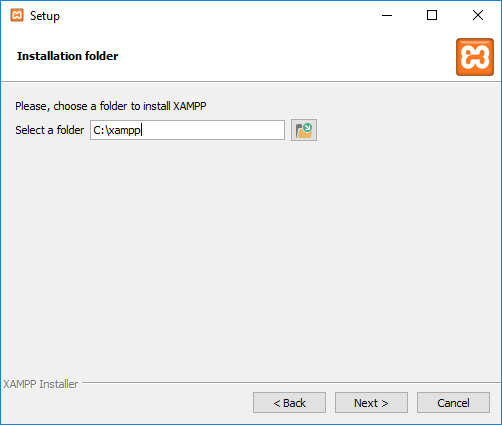
\includegraphics[scale=0.4]{pics/xampp4}  %el parámetro scale permite agrandar o achicar la imagen. En el nombre de archivo puede especificar directorios
		\caption{Paso 3 instalación XAMPP} \label{fig:XAMPP4}
	\end{figure}
	
	\item Ya comienza a instalarse.
	
	\begin{figure}[H] %con el [H] le obligamos a situar aquí la figura
		\centering
		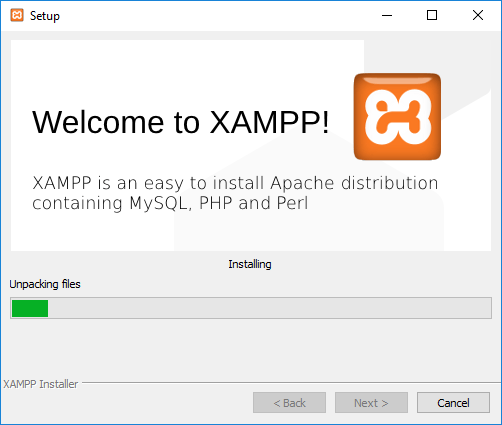
\includegraphics[scale=0.4]{pics/xampp5}  %el parámetro scale permite agrandar o achicar la imagen. En el nombre de archivo puede especificar directorios
		\caption{Paso 4 instalación XAMPP} \label{fig:XAMP5}
	\end{figure}
	
	\item Debemos permitir el acceso a través del firewall de Windows.
	
	\begin{figure}[H] %con el [H] le obligamos a situar aquí la figura
		\centering
		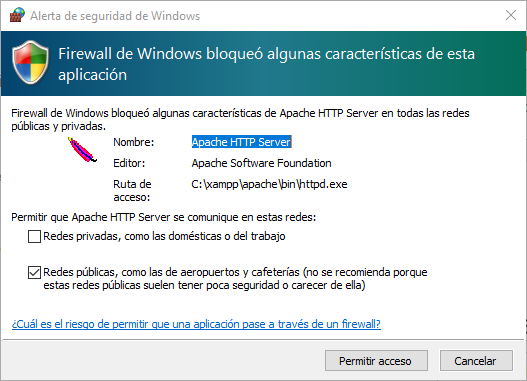
\includegraphics[scale=0.4]{pics/xampp6}  %el parámetro scale permite agrandar o achicar la imagen. En el nombre de archivo puede especificar directorios
		\caption{Paso 5 instalación XAMPP} \label{fig:XAMP6}
	\end{figure}
	
	\item Una ha terminado de instalarse se nos abrirá la interfaz del panel de Control de XAMPP y debemos darle a start en Apache para ejecutar el servicio.
	
	\begin{figure}[H] %con el [H] le obligamos a situar aquí la figura
		\centering
		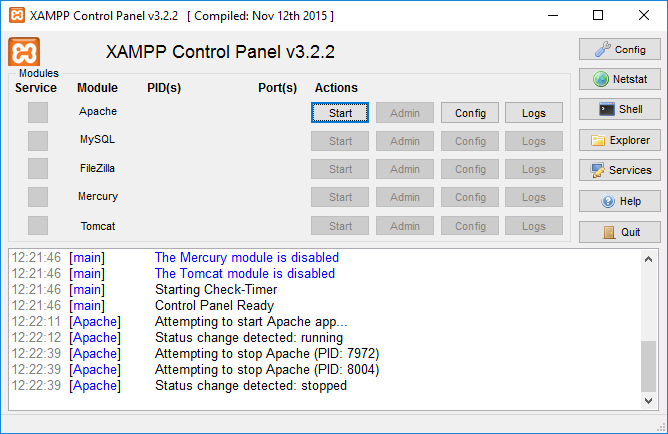
\includegraphics[scale=0.4]{pics/xampp7}  %el parámetro scale permite agrandar o achicar la imagen. En el nombre de archivo puede especificar directorios
		\caption{Panel Control XAMPP} \label{fig:XAMP7}
	\end{figure}
	
\end{enumerate}

Una vez tenemos apache instalado ya contamos con su herramienta ab (Apache Benchmark) para poder realizar las pruebas a las maquinas virtuales desde el anfitrión.

Antes de empezar configuraré la pagina index.html para el benchmark en los tres servidores para que estén en igualdad de condiciones.\\
El archivo index.html que utilizaré contiene html con un un titulo y h1,h2,h3,h4,h5 y h6 con texto generado en latin.\\

Al igual que en el ejercicio anterior mandare ejecutaré el benchmark con:\\

\begin{center}
	\textit{ab -n 5000 -c 50 http://host/index.html }
\end{center}

Generará 5000 peticiones a cada servidor y las mandará en paquetes de 50.

\begin{enumerate}
	\item \textbf{Benchmark Ubuntu}:
		Ejecutaré \textit{ab -n 5000 -c 50 http://192.168.23.2/index.html} dos veces para verificar que se obtiene un tiempo medio.
		
		\begin{figure}[H] %con el [H] le obligamos a situar aquí la figura
			\centering
				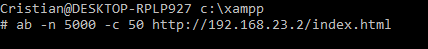
\includegraphics[scale=0.4]{pics/xamppUbu1}  %el parámetro scale permite agrandar o achicar la imagen. En el nombre de archivo puede especificar directorios
			\caption{Benchmark Ubuntu 1} \label{fig:ubu1}
		\end{figure}
	
		Ejecución 1:
		
		\begin{figure}[H] %con el [H] le obligamos a situar aquí la figura
			\centering
			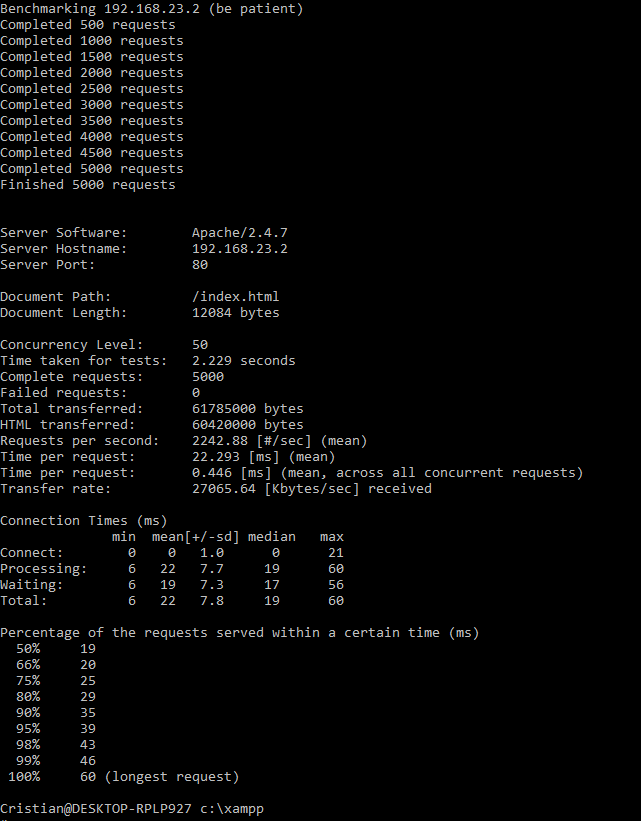
\includegraphics[scale=0.4]{pics/xamppUbu2}  %el parámetro scale permite agrandar o achicar la imagen. En el nombre de archivo puede especificar directorios
			\caption{Benchmark Ubuntu 2} \label{fig:ubu2}
		\end{figure}
	
			Ejecución 2:
	
		\begin{figure}[H] %con el [H] le obligamos a situar aquí la figura
			\centering
			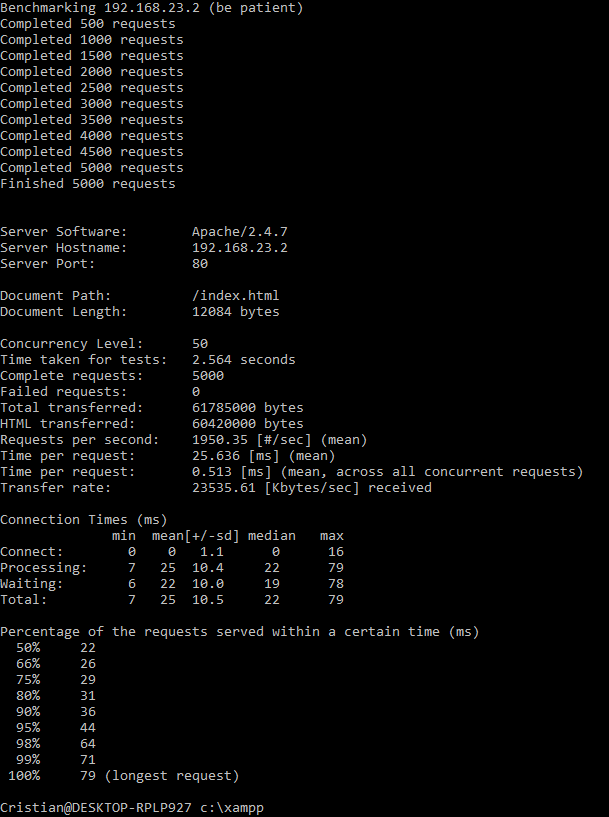
\includegraphics[scale=0.4]{pics/xamppUbu3}  %el parámetro scale permite agrandar o achicar la imagen. En el nombre de archivo puede especificar directorios
			\caption{Benchmark Ubuntu 3} \label{fig:ubu3}
		\end{figure}
	\item \textbf{Benchmark CentOS}:
		Ejecutaré \textit{ab -n 5000 -c 50 http://192.168.23.3/index.html} dos veces para verificar que se obtiene un tiempo medio.
		
		\begin{figure}[H] %con el [H] le obligamos a situar aquí la figura
			\centering
			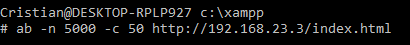
\includegraphics[scale=0.4]{pics/xamppCent1}  %el parámetro scale permite agrandar o achicar la imagen. En el nombre de archivo puede especificar directorios
			\caption{Benchmark CentOS 1} \label{fig:cen1}
		\end{figure}
		
		Ejecución 1:
		
		\begin{figure}[H] %con el [H] le obligamos a situar aquí la figura
			\centering
			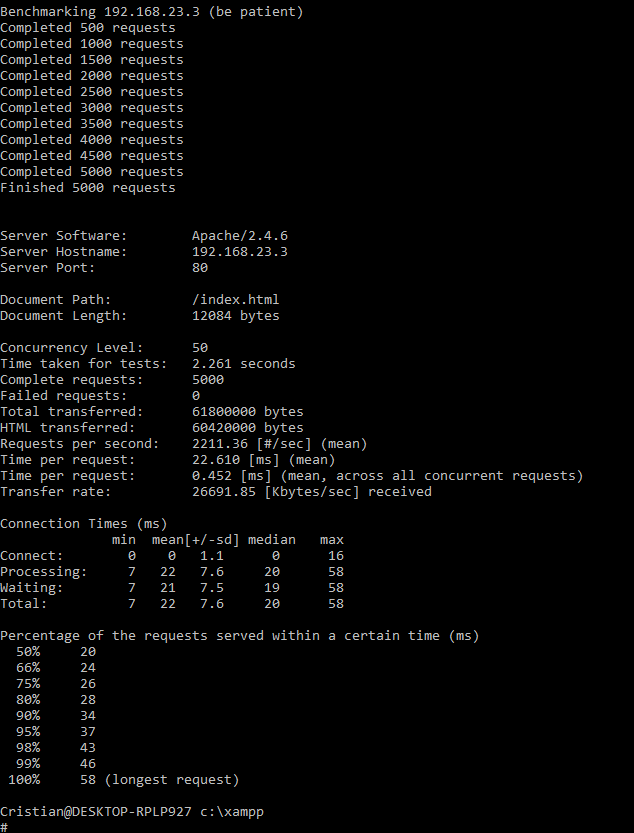
\includegraphics[scale=0.4]{pics/xamppCent2}  %el parámetro scale permite agrandar o achicar la imagen. En el nombre de archivo puede especificar directorios
			\caption{Benchmark CentOS 2} \label{fig:cen2}
		\end{figure}
		
		Ejecución 2:
		
		\begin{figure}[H] %con el [H] le obligamos a situar aquí la figura
			\centering
			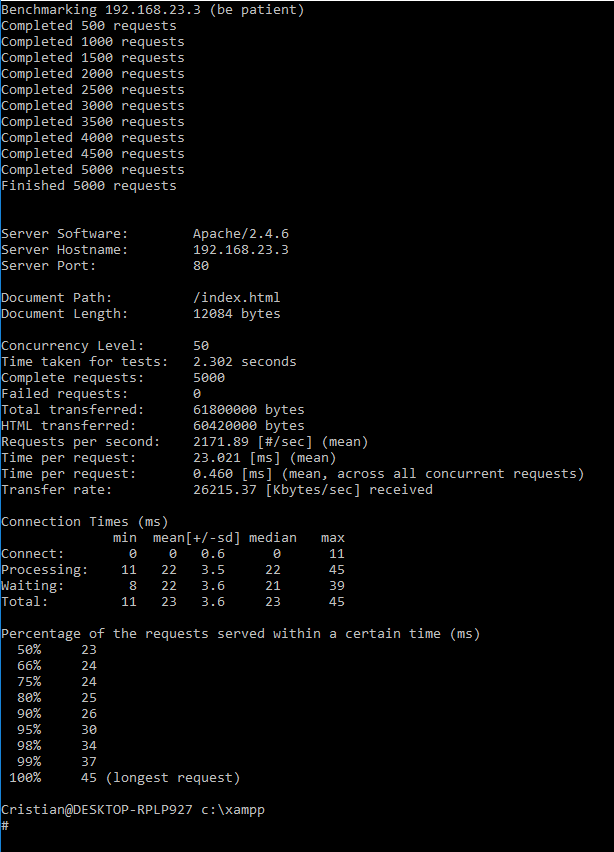
\includegraphics[scale=0.4]{pics/xamppCent3}  %el parámetro scale permite agrandar o achicar la imagen. En el nombre de archivo puede especificar directorios
			\caption{Benchmark CentOS 3} \label{fig:cen3}
		\end{figure}
	
	\item \textbf{Benchmark Windows Server}:
	
			Ejecutaré \textit{ab -n 5000 -c 50 http://192.168.23.4/index.html} dos veces para verificar que se obtiene un tiempo medio.
		
		\begin{figure}[H] %con el [H] le obligamos a situar aquí la figura
			\centering
			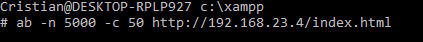
\includegraphics[scale=0.4]{pics/xamppWin1}  %el parámetro scale permite agrandar o achicar la imagen. En el nombre de archivo puede especificar directorios
			\caption{Benchmark Windows 1} \label{fig:win1}
		\end{figure}
		
		Ejecución 1:
		
		\begin{figure}[H] %con el [H] le obligamos a situar aquí la figura
			\centering
			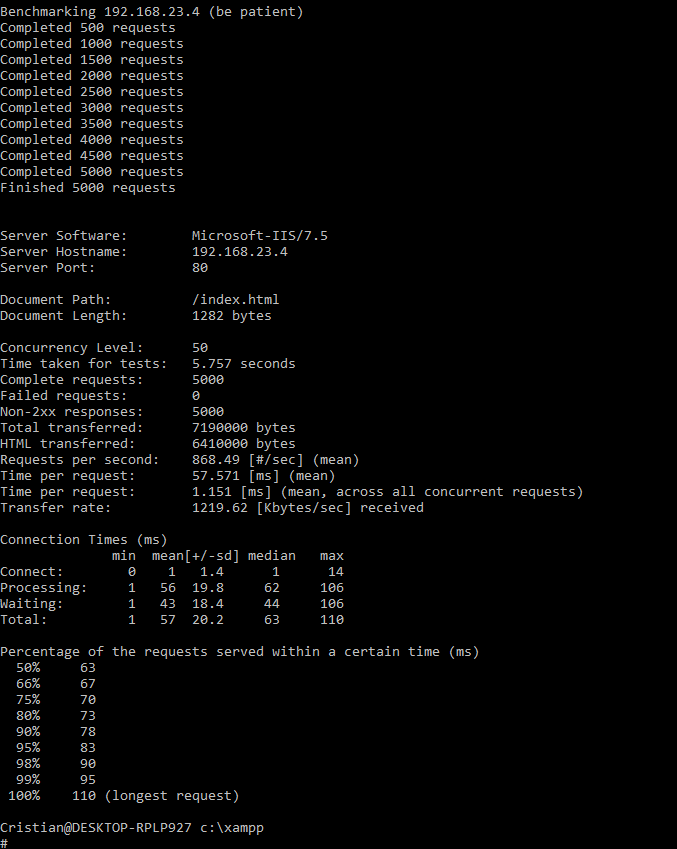
\includegraphics[scale=0.4]{pics/xamppWin2}  %el parámetro scale permite agrandar o achicar la imagen. En el nombre de archivo puede especificar directorios
			\caption{Benchmark Windows 2} \label{fig:win2}
		\end{figure}
		
		Ejecución 2:
		
		\begin{figure}[H] %con el [H] le obligamos a situar aquí la figura
			\centering
			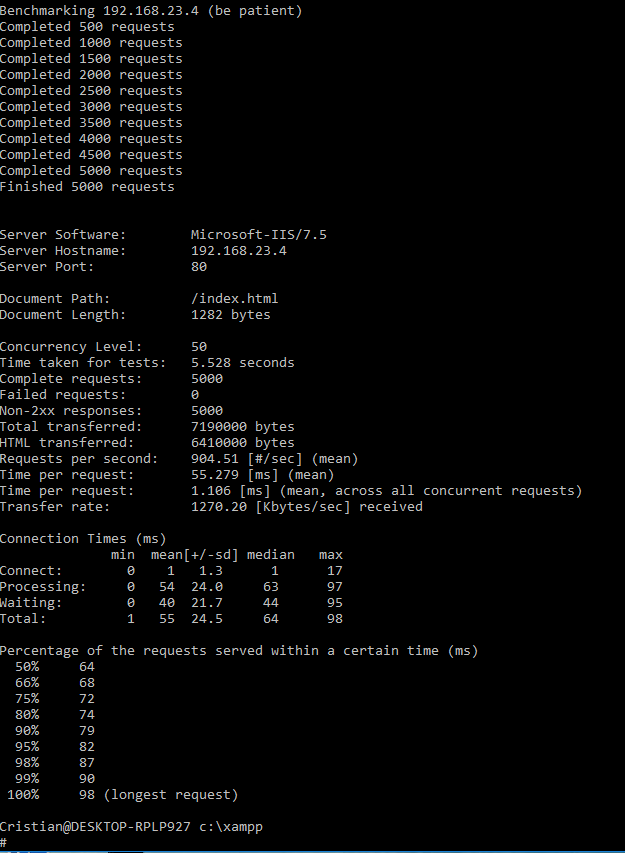
\includegraphics[scale=0.4]{pics/xamppWin3}  %el parámetro scale permite agrandar o achicar la imagen. En el nombre de archivo puede especificar directorios
			\caption{Benchmark Windows 3} \label{fig:win3}
		\end{figure}
	
\end{enumerate}

\textbf{Conclusión:} Obtenemos la siguiente tabla con los tiempos de conexión en milisegundos.\\

\begin{center}
		\begin{tabular}{|c|c|c|c|}
		\hline 
		& Ejecución 1 & Ejecución 2 & Media \\ 
		\hline 
		Ubuntu & 19 & 22 & 20.5 \\ 
		\hline 
		CentOS & 20 & 23 & 21.5 \\ 
		\hline 
		Windows & 63 & 64 & 63.5 \\ 
		\hline 
	\end{tabular} 
\end{center}

Como podemos apreciar el servidor que mas rápido ha sido es Ubuntu, seguido de CentOS y finalmente Windows Server.





%----------------------------------------------------------------------------------------
%	Cuestión 4
%----------------------------------------------------------------------------------------
\section[Cuestión 4]{Instale y siga el tutorial en	 realizando capturas de pantalla y comentándolas. En vez de usar la web de jmeter, haga el experimento usando sus máquinas virtuales ¿coincide con los resultados de ab?}

%----------------------------------------------------------------------------------------
%	Cuestión 5
%----------------------------------------------------------------------------------------
\section[Cuestión 5]{ Programe un benchmark usando el lenguaje que desee. El benchmark debe incluir, Objetivo del benchmark, Métricas (unidades, variables, puntuaciones, etc.), Instrucciones para su uso, Ejemplo de uso analizando los resultados.}


\bibliography{citas} %archivo citas.bib que contiene las entradas 
\bibliographystyle{plain} % hay varias formas de citar

\end{document}
\grid
